\section{Audit results}
\label{sec:audit}

\subsection{The evidence base}
The 32 core papers span 2010--2026, and 21 of them appeared in 2022 or later. 22 are peer-reviewed, 9 are preprints and 1 is grey literature.

\begin{itemize}
  \item \textbf{Security dominates.} 24 papers are on security telemetry. Network flows (S1) are the largest cluster, with 10 papers.
  \item \textbf{Systems telemetry is thin.} Only 8 papers are on systems telemetry, and 4 of those (I1) evaluate on generic multivariate benchmarks such as SMD rather than on an operational system.
  \item \textbf{Use.} Topology is used for detection in 14 papers, for visual exploration in 8, as a component inside a larger learned model in 8, for efficiency in 1, and the use is unclear in 1.
\end{itemize}

\subsection{Outcomes: how often does topology win, and against what?}
Figure~\ref{fig:evidence} and Table~\ref{tab:outcomes} summarise the outcomes. Across all 32 papers, topology helped in 5, tied in 4, gave mixed results in 2 and lost in 3. In 12 papers it was never compared with anything. For the remaining 6, the outcome is known only from an abstract or from released code (3), or could not be determined (3).

The headline counts hide the main problem: \emph{what} topology was compared against. Panel~(b) of Figure~\ref{fig:evidence} splits the 14 full-text papers that make any comparison by how they isolate topology. Only the four replacement studies (group A) can show that topology itself adds value. Of those, two lost, one tied and one gave a weak win.

\begin{figure}[ht]
\centering
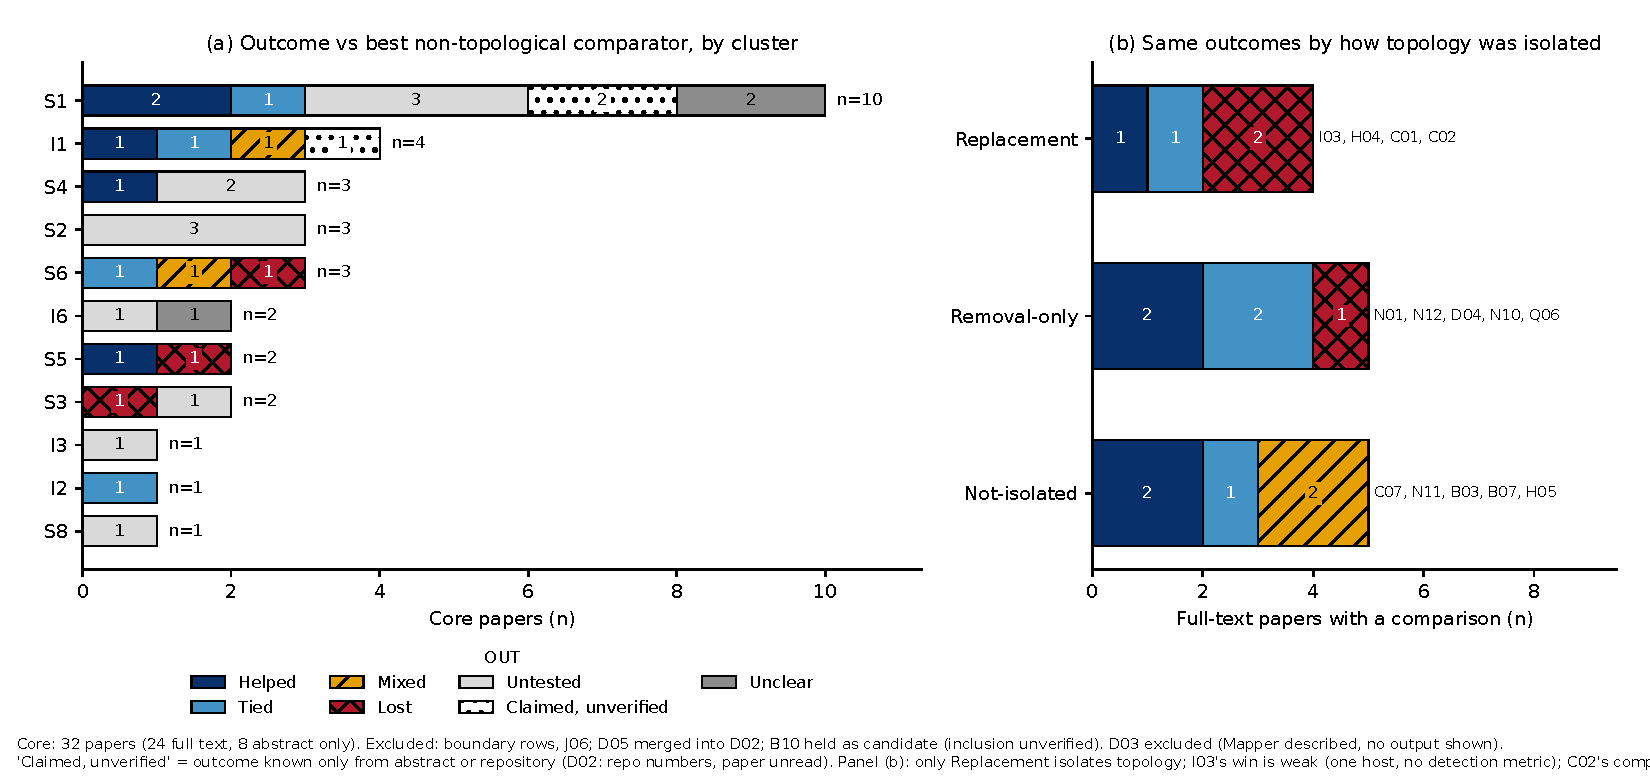
\includegraphics[width=\linewidth]{fig1_evidence_map.pdf}
\caption{Evidence map of the 32 core papers. (a) Outcome against the best non-topological comparator in the same paper, by cluster. (b) Outcomes of the 14 full-text papers that make a comparison, split by how they isolate topology. Only \emph{Replacement} is a swap test.}
\label{fig:evidence}
\end{figure}

\begin{table}[ht]
\centering\small
\caption{The 32 core papers grouped by study design (paper-by-paper dossier).}
\label{tab:outcomes}
\begin{tabularx}{\linewidth}{@{}lL{3.5cm}rYL{3.2cm}@{}}
\toprule
Group & Design & $n$ & Papers & Outcome \\
\midrule
A & Topology swapped for cheap features & 4 & C01, C02, H04, I03 & 2 lost, 1 tied, 1 weak win \\
B & Topology only removed & 5 & N01, N12, D04, N10, Q06 & 2 helped, 2 tied, 1 lost \\
C & Compared with other people's systems & 5 & C07, N11, B03, B07, H05 & 2 helped, 1 tied, 2 mixed \\
D & No comparison & 10 & B01, B08, D01, I02, J07, G01, I04, J05, C06, Q05 & untested \\
E & Abstract or code only & 8 & D02, N03, C08; N07, N09, B09; B05, B06 & 3 claimed, 3 unclear, 2 untested \\
\bottomrule
\end{tabularx}
\end{table}

\paragraph{Group A: the four swap tests.}
\begin{itemize}
  \item \textbf{\rec{C01}, host logs.} Persistent-homology features were compared with count features, using the same random forest and 10-fold cross-validation, on two synthetic log datasets and two graph constructions. Topology scored below the best non-topological feature set in all four settings, by 3.6 to 9.1 F1 points. For example, it reached 66.56 against 72.53 for counts.
    \emph{Caveat:} the data is synthetic and balanced, and the random folds likely overlap between training and test.
    This is the cleanest test in the literature, and topology lost.
  \item \textbf{\rec{C02}, malware.} Persistence-diagram features were swapped for PCA, UMAP and t-SNE features under the same tree learners, on CIC-MalMem-2022. The diagram features reached a detection rate of ``over 80\% on average''; UMAP and t-SNE reached 99--100\%. Extracting diagram features took 24.7\,s, against 1.08\,s for PCA.
    \emph{Caveat:} the diagram arm appears to be trained on homology-group labels rather than malware labels, so the comparison is not like-for-like.
    We code this as a loss of doubtful validity.
  \item \textbf{\rec{H04}, TADA on Exathlon (big-data jobs).} TADA ranked first on 5 of the 15 tabulated problems (by Range PR-AUC). The paper's own statistical ranking places it third, behind a non-topological method and Atol-IF, a related topological pipeline. We code this as a tie.
  \item \textbf{\rec{I03}, zigzag persistence on DARPA OpTC flows.} An autoencoder on zigzag features was compared with the same autoencoder on the authors' own summary statistics (edges, vertices, components, diameter). For one host, the malicious-to-benign reconstruction-loss ratio was about 36 with zigzag features and about 7.5 with summary statistics, and the zigzag spike matched the first attack in time.
    \emph{Caveats:} only one host is tabulated, with one seed, on one day. There is no threshold and no detection metric. The second attack group was missed. OpTC's benign activity is simulated.
    This is the only swap-test win, and it is weak. E4 re-tests the idea on CTU-13.
\end{itemize}

\paragraph{Group B: removal only.} These papers delete the topology branch and show that the full model scores higher:
\begin{itemize}
  \item \rec{N01}: F1 0.994 against 0.930 without persistent homology, in a single run;
  \item \rec{N12}: +0.5 to +2.2 F1 points;
  \item \rec{D04}: +3.8 average F1 points over the version without topology.
\end{itemize}
This shows that the model benefits from the extra input. It does not show that topology beats a cheap input of the same size. Against external baselines, the same papers are close. TopoGDN (D04) beats TranAD by 0.54 F1 points on SMD and 0.85 on MSL, in single runs without variance. Its removal ablation also disagrees with its own main table on SWaT. In \rec{N10}, the hybrid model, an LSTM alone and an SVM all score F1 = 1.000 on CIC-IDS2017. In \rec{Q06}, adding TDA \emph{halved} accuracy in the hardest setting (34\% against 68\%).

\paragraph{Group C: other people's systems.} These papers compare against baselines that differ in learner, tuning or data split:
\begin{itemize}
  \item \rec{C07}: gradient boosting on topological features against a graph neural network on raw call graphs;
  \item \rec{N11}: an oversampler against other learners;
  \item \rec{B03}: accuracy against numbers quoted from the literature for different windows.
\end{itemize}
Their wins and ties cannot be credited to topology. \rec{H05} has the best average rank over 18 univariate datasets but is not significantly better than the top methods. \rec{B07} is mixed.

\paragraph{Groups D and E.} The 10 untested papers are mostly exploratory: Mapper views of darknet traffic, log analytics and hypergraph motifs inspected by hand. Their interpretations rest on inspection, not on detection results. The 8 papers in group E could be assessed only from their abstracts or released code. One of them, TAME (D02), is the code-audit and replication case in Sections~\ref{sec:code} and~\ref{sec:exp}.

\subsection{Rigour}
Figure~\ref{fig:rigour} scores every core paper on R1--R13. Five patterns stand out.

\begin{itemize}
  \item \textbf{Isolation is rare.} Only 3 papers (9\%) have a fully matched non-topological baseline (R1), and only 3 run a full replacement ablation (R2). A fourth, C02, attempts one, but the comparison is not like-for-like.
  \item \textbf{Leakage is not ruled out anywhere.} No paper meets R3 (a time- or entity-separated split with everything fitted on training data only). Only one paper meets R4: \rec{C01} chooses its threshold without test labels or test prevalence. For 14 papers, R4 does not apply.
  \item \textbf{Uncertainty and stress tests are missing.} No paper measures uncertainty across independent units such as hosts, days or scenarios (R6). None tests robustness to noise, drift or missing data (R8). None tests an adversary who knows the method (R9): 25 papers do not, and 7 cannot be assessed.
  \item \textbf{Benchmarks are taken at face value.} No paper fully meets R10.
    \begin{itemize}
      \item Two network papers use CIC-IDS2017 without saying they use a corrected version~\cite{N10,N11}, despite documented labelling errors~\cite{Q03}.
      \item Three systems papers (D02, D04, N12) use SMD, SMAP/MSL or Yahoo without discussing published critiques of those benchmarks~\cite{Q04}.
    \end{itemize}
    Only one paper (H04) reports a prevalence-aware metric (R5).
  \item \textbf{Little can be re-run.} Code is released for 4 papers (12.5\%), and data is available for 14 (44\%).
\end{itemize}

\begin{figure}[p]
\centering
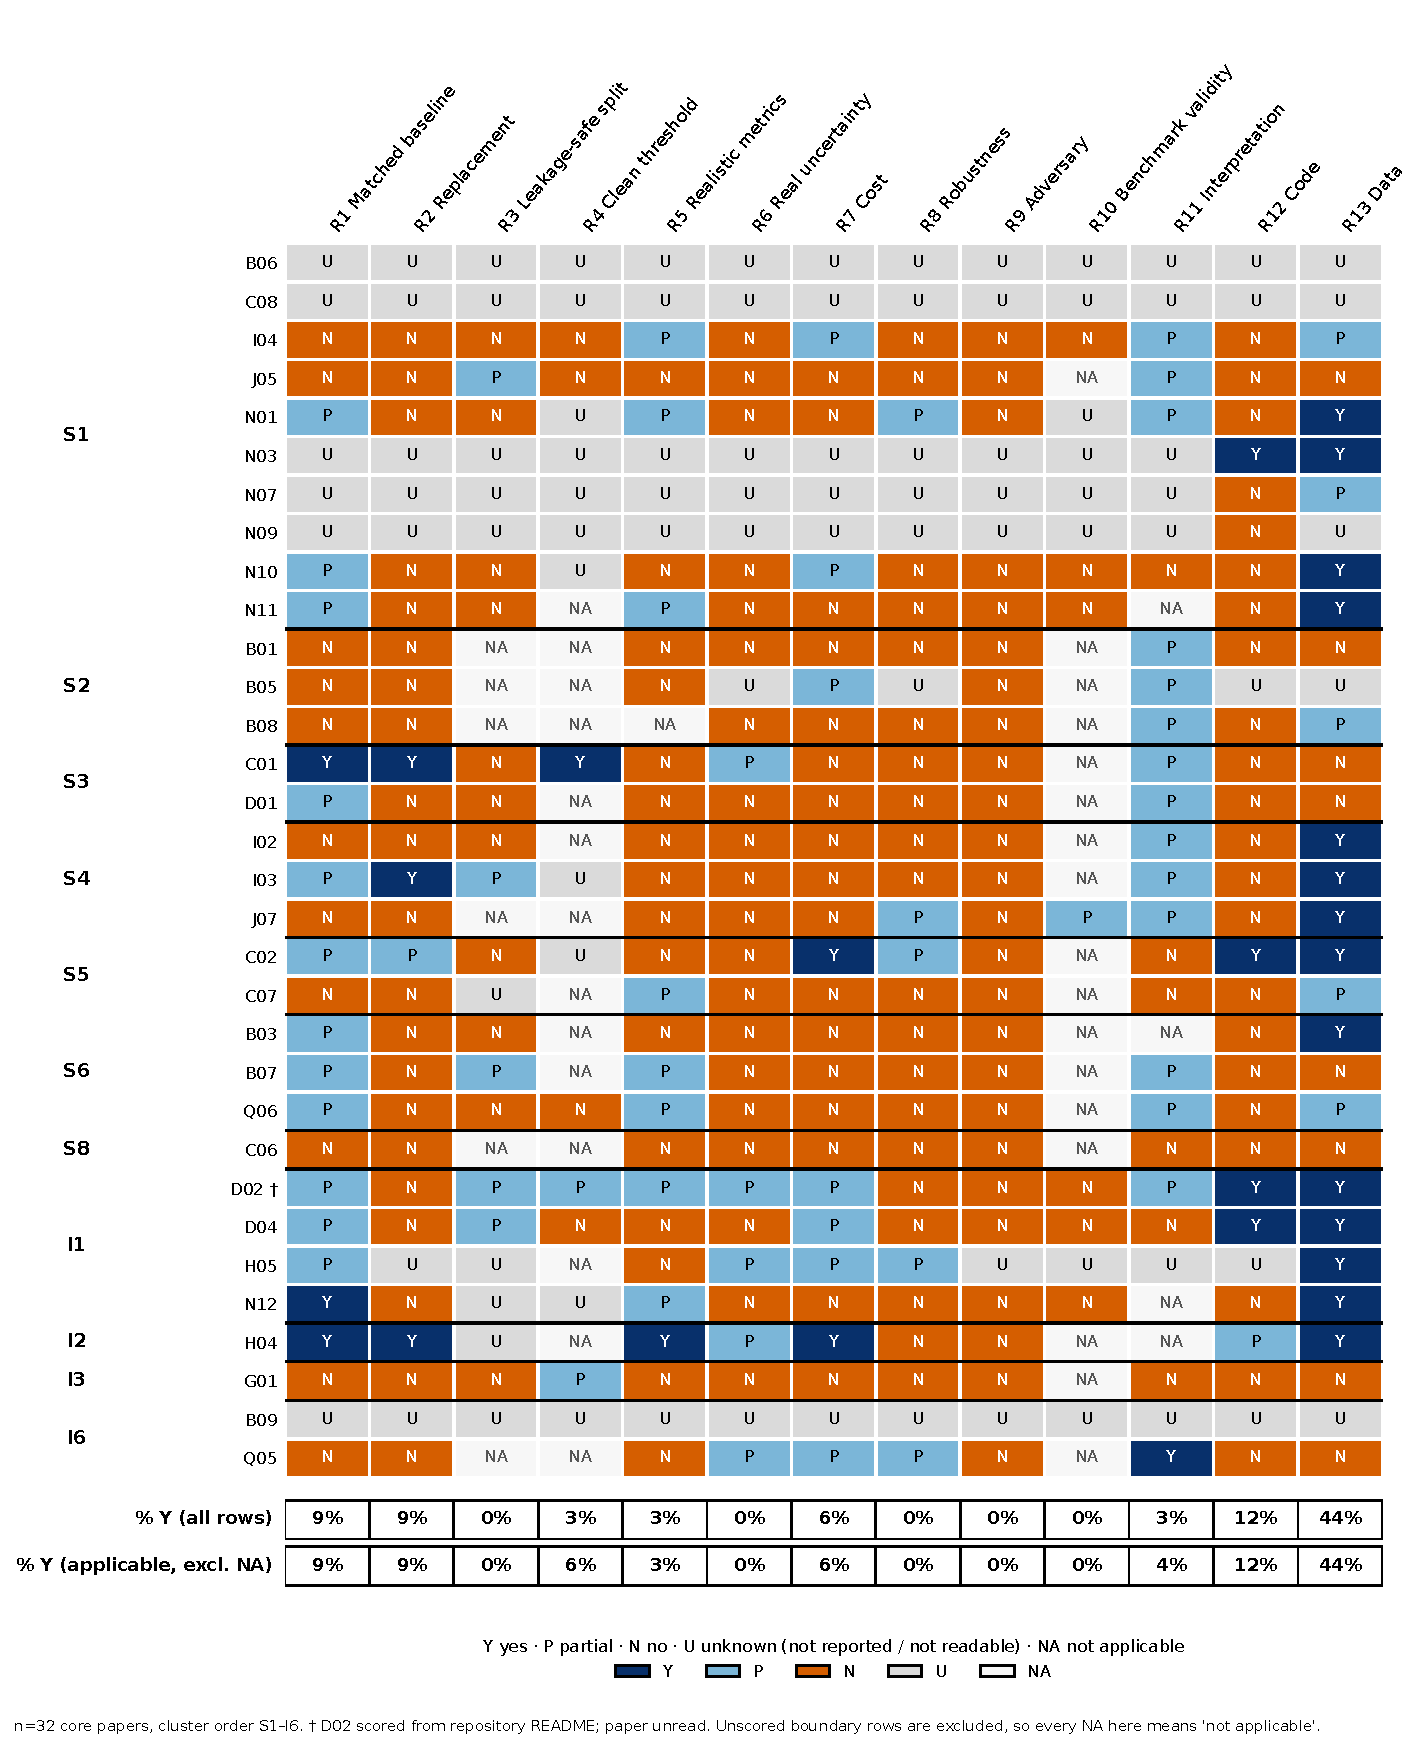
\includegraphics[width=\linewidth,height=0.86\textheight,keepaspectratio]{fig2_rigor_heatmap.pdf}
\caption{Rigour heatmap: R1--R13 for the 32 core papers, grouped by cluster. The bottom rows give the share of papers scoring Y. Every NA means ``not applicable''. D02 (\dag) was scored from its repository README because the paper was not readable.}
\label{fig:rigour}
\end{figure}

\subsection{What the audit can and cannot conclude}
The audit shows that the central claim, that topology adds detection value beyond cheap features, is \emph{almost untested}. It does not show that the claim is false.
\begin{itemize}
  \item The two swap-test losses come from synthetic data (C01) and from a doubtful comparison (C02).
  \item The single win (I03) rests on one host.
  \item Eight papers could be read only as abstracts.
  \item The coding was done by one person with AI assistance, and its reliability is estimated only by the self re-check (Section~\ref{sec:recheck}).
\end{itemize}
The obvious next step is therefore to run the missing test ourselves. That is the purpose of the preregistered experiments in Section~\ref{sec:exp}.
